% This file was created with tikzplotlib v0.10.1.
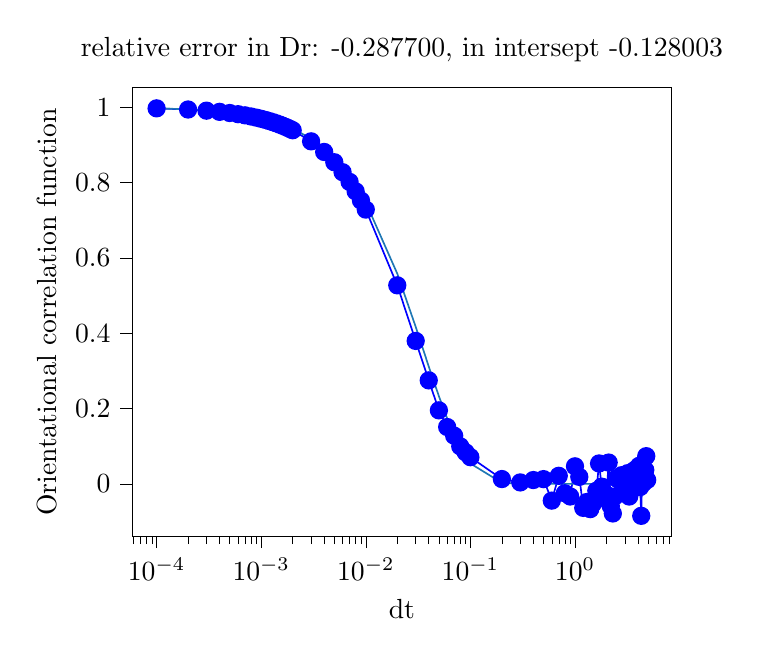
\begin{tikzpicture}

\definecolor{darkgray176}{RGB}{176,176,176}
\definecolor{steelblue31119180}{RGB}{31,119,180}

\begin{axis}[
log basis x={10},
tick align=outside,
tick pos=left,
title={relative error in Dr: -0.287700, in intersept -0.128003},
x grid style={darkgray176},
xlabel={dt},
xmin=5.8276061909058e-05, xmax=8.40825519000689,
xmode=log,
xtick style={color=black},
y grid style={darkgray176},
ylabel={Orientational correlation function},
ymin=-0.138791889328458, ymax=1.05117859332981,
ytick style={color=black}
]
\addplot [semithick, blue, mark=*, mark size=3, mark options={solid}]
table {%
0.0001 0.996874319930448
0.0002 0.993753638992955
0.0003 0.990648385121479
0.0004 0.987556156010123
0.0005 0.984468328080447
0.0006 0.981381734367307
0.0007 0.978306243105779
0.0008 0.97523327095795
0.0009 0.97215449236398
0.001 0.969097383036741
0.0011 0.966037289703948
0.0012 0.962992411201345
0.0013 0.959960810654644
0.0014 0.956924286995569
0.0015 0.953886329000577
0.0016 0.950845307404892
0.0017 0.947818448075686
0.0018 0.944775431786025
0.0019 0.941747947240794
0.002 0.93873552856681
0.003 0.909273650355168
0.004 0.881108484984952
0.005 0.853825347171386
0.006 0.827371448154515
0.007 0.801655449903083
0.008 0.776444490321183
0.009 0.752091567364772
0.01 0.728158448265329
0.02 0.527084628053719
0.03 0.379491460469431
0.04 0.274798016096666
0.05 0.195228998411697
0.06 0.150974495919378
0.07 0.127880123564861
0.08 0.0997042841116788
0.09 0.0838908736485968
0.1 0.0708720455443572
0.2 0.0128578546772169
0.3 0.00396198532793916
0.4 0.0102937522332671
0.5 0.0127330770591652
0.6 -0.0443937101483357
0.7 0.0214521398805833
0.8 -0.0247189809656514
0.9 -0.0334108352611225
1 0.0466476804323349
1.1 0.0186839523006204
1.2 -0.0635807763087332
1.3 -0.047984567704674
1.4 -0.066946080148079
1.5 -0.0507870804104135
1.6 -0.0183216956776642
1.7 0.0542877065614584
1.8 -0.00729238886897958
1.9 -0.0370813600025087
2 -0.0283370613566181
2.1 0.0566533984203141
2.2 -0.0591909026896688
2.3 -0.0784294704821597
2.4 -0.03344008379972
2.5 0.0149736799632406
2.6 0.0112772331944409
2.7 0.0187246295235108
2.8 0.0231665813253398
2.9 -0.0160820954830479
3 -0.00510396182414909
3.1 0.0151695798888382
3.2 0.0285877985873751
3.3 -0.033479014781865
3.4 -0.0199449942313608
3.5 0.00772682096444017
3.6 0.0159446128728458
3.7 0.0366284477614433
3.8 0.00465260034655319
3.9 0.0370882309186447
4 -0.00599469224848418
4.1 0.0478612141340291
4.2 -0.0083747513044814
4.3 -0.0847023219349006
4.4 0.0364375045955743
4.5 0.00224115765314868
4.6 0.00992129911990771
4.7 0.036656577182127
4.8 0.073662040538887
4.9 0.010441017483902
};
\addplot [semithick, steelblue31119180]
table {%
0.0001 0.997089025936249
0.0002 0.994186525642498
0.0003 0.991292474451822
0.0004 0.988406847769101
0.0005 0.985529621070811
0.0006 0.982660769904815
0.0007 0.979800269890157
0.0008 0.97694809671685
0.0009 0.974104226145677
0.001 0.971268634007976
0.0011 0.968441296205444
0.0012 0.965622188709925
0.0013 0.962811287563207
0.0014 0.960008568876824
0.0015 0.957214008831845
0.0016 0.954427583678676
0.0017 0.951649269736859
0.0018 0.948879043394868
0.0019 0.946116881109908
0.002 0.94336275940772
0.003 0.916258658703931
0.004 0.889933295837348
0.005 0.864364296606157
0.006 0.839529929649928
0.007 0.815409087979898
0.008 0.791981271039925
0.009 0.769226567282849
0.01 0.747125637247457
0.02 0.558196717832419
0.03 0.417043078519985
0.04 0.311583575798885
0.05 0.232792077624583
0.06 0.173924929341426
0.07 0.129943773667432
0.08 0.0970843247076193
0.09 0.0725341879639191
0.1 0.0541921514047699
0.2 0.0029367892738775
0.3 0.000159150928973874
0.4 8.62473123916195e-06
0.5 4.67392741138113e-07
0.6 2.53290181932471e-08
0.7 1.37263398886261e-09
0.8 7.4385988947776e-11
0.9 4.03113677545142e-12
1 2.18455974468599e-13
1.1 1.18385992436788e-14
1.2 6.41559162633841e-16
1.3 3.47674712765705e-17
1.4 1.88412406738089e-18
1.5 1.02104736724876e-19
1.6 5.53327535173865e-21
1.7 2.99860095625702e-22
1.8 1.62500637023969e-23
1.9 8.80625912497442e-25
2 4.77230127810253e-26
2.1 2.58621273412109e-27
2.2 1.40152432052433e-28
2.3 7.59516181753216e-30
2.4 4.11598159159435e-31
2.5 2.23053897590927e-32
2.6 1.20877705896715e-33
2.7 6.55062293941603e-35
2.8 3.54992350128392e-36
2.9 1.92377991856926e-37
3 1.04253772616563e-38
3.1 5.64973623015521e-40
3.2 3.06171361181585e-41
3.3 1.65920847609569e-42
3.4 8.99160769486551e-44
3.5 4.87274565572452e-45
3.6 2.64064570331958e-46
3.7 1.43102271760647e-47
3.8 7.75501997761952e-49
3.9 4.20261216774172e-50
4 2.2774859488979e-51
4.1 1.23421863364909e-52
4.2 6.68849630613008e-54
4.3 3.6246400449205e-55
4.4 1.96427042102118e-56
4.5 1.06448040055892e-57
4.6 5.76864830344984e-59
4.7 3.12615462261427e-60
4.8 1.69413044623436e-61
4.9 9.18085736417613e-63
};
\end{axis}

\end{tikzpicture}
